%% 
%% Copyright 2007-2020 Elsevier Ltd
%% 
%% This file is part of the 'Elsarticle Bundle'.
%% ---------------------------------------------
%% 
%% It may be distributed under the conditions of the LaTeX Project Public
%% License, either version 1.2 of this license or (at your option) any
%% later version.  The latest version of this license is in
%%    http://www.latex-project.org/lppl.txt
%% and version 1.2 or later is part of all distributions of LaTeX
%% version 1999/12/01 or later.
%% 
%% The list of all files belonging to the 'Elsarticle Bundle' is
%% given in the file `manifest.txt'.
%% 

%% Template article for Elsevier's document class `elsarticle'
%% with numbered style bibliographic references
%% SP 2008/03/01
%%
%% 
%%
%% $Id: elsarticle-template-num.tex 190 2020-11-23 11:12:32Z rishi $
%%
%%
\documentclass[preprint,12pt]{elsarticle}

%% Use the option review to obtain double line spacing
%% \documentclass[authoryear,preprint,review,12pt]{elsarticle}

%% Use the options 1p,twocolumn; 3p; 3p,twocolumn; 5p; or 5p,twocolumn
%% for a journal layout:
%% \documentclass[final,1p,times]{elsarticle}
%% \documentclass[final,1p,times,twocolumn]{elsarticle}
%% \documentclass[final,3p,times]{elsarticle}
%% \documentclass[final,3p,times,twocolumn]{elsarticle}
%% \documentclass[final,5p,times]{elsarticle}
%% \documentclass[final,5p,times,twocolumn]{elsarticle}

%% For including figures, graphicx.sty has been loaded in
%% elsarticle.cls. If you prefer to use the old commands
%% please give \usepackage{epsfig}

%% The amssymb package provides various useful mathematical symbols
\usepackage{amssymb}
\usepackage{tikz}
\usepackage{amsmath}
\usepackage{subcaption}
\usepackage{url}
%% The amsthm package provides extended theorem environments
%% \usepackage{amsthm}

%% The lineno packages adds line numbers. Start line numbering with
%% \begin{linenumbers}, end it with \end{linenumbers}. Or switch it on
%% for the whole article with \linenumbers.
%% \usepackage{lineno}

\journal{Journal of Chemometrics}

\begin{document}

\begin{frontmatter}

%% Title, authors and addresses

%% use the tnoteref command within \title for footnotes;
%% use the tnotetext command for theassociated footnote;
%% use the fnref command within \author or \address for footnotes;
%% use the fntext command for theassociated footnote;
%% use the corref command within \author for corresponding author footnotes;
%% use the cortext command for theassociated footnote;
%% use the ead command for the email address,
%% and the form \ead[url] for the home page:
%% \title{Title\tnoteref{label1}}
%% \tnotetext[label1]{}
%% \author{Name\corref{cor1}\fnref{label2}}
%% \ead{email address}
%% \ead[url]{home page}
%% \fntext[label2]{}
%% \cortext[cor1]{}
%% \affiliation{organization={},
%%             addressline={},
%%             city={},
%%             postcode={},
%%             state={},
%%             country={}}
%% \fntext[label3]{}

\title{An alignment-agnostic methodology for the analysis of designed separations data}

%% use optional labels to link authors explicitly to addresses:
%% \author[label1,label2]{}
%% \affiliation[label1]{organization={},
%%             addressline={},
%%             city={},
%%             postcode={},
%%             state={},
%%             country={}}
%%
%% \affiliation[label2]{organization={},
%%             addressline={},
%%             city={},
%%             postcode={},
%%             state={},
%%             country={}}

\author{Michael Sorochan Armstrong}
\author{Jos\'e Camacho}
\address{Computational Data Science (CoDaS) Lab, Department of Signal Theory, Networks and Communication - University of Granada,%Department and Organization
            %C/ Periodista Daniel Saucedo Aranda S/N CP:18071 Granada (Granada)
            C/ Periodista Daniel Saucedo Aranda, 
            Granada,
            18071, 
            Andalusia,
            Spain}
\begin{abstract}
%% Text of abstract
Chemical separations data are typically analysed in the time domain using methods that integrate the discrete elution bands. Integrating the same chemical components across several samples must account for retention time drift over the course of an entire experiment as the physical characteristics of the separation are altered through several cycles of use. Failure to consistently integrate the components within a matrix of $M \times N$ samples and variables create artifacts that have a profound effect on the analysis and interpretation of the data. This work presents an alternative where the raw separations data are analysed in the frequency domain to account for the offset of the chromatographic peaks as a matrix of complex Fourier coefficients. We present a generalization of the permutation testing, and visualization steps in ANOVA-Simultaneous Component Analysis (ASCA) to handle complex matrices, and use this method to analyze a synthetic dataset with known significant factors and compare the interpretation of a real dataset via its peak table and frequency domain representations.

\end{abstract}

%%Graphical abstract


%%Research highlights
\begin{highlights}
\item Raw GC-FID signal from a designed experimental dataset is treated with a Fast Fourier Transform (FFT) and analysed using a generalization of ANOVA-Simultaneous Component Analysis (ASCA) to handle complex data.
\item The results of the FFT-ASCA analysis are largely consistent with the analysis using the peak table data. This is confirmed using a demonstration with synthetic data.
\end{highlights}

\begin{keyword}
%% keywords here, in the form: keyword \sep keyword
ANOVA \sep ASCA \sep chromatographic data

\end{keyword}

\end{frontmatter}

%% \linenumbers

%% main text
\section{Introduction}
\label{sec:sample1}
\subsection{Challenges with peak table analysis}
Chromatographic separations enable detailed analyses of chemical mixtures, providing valuable information for researchers interrogating complex systems. For a multivariate analysis, several samples are collected and discrete chemical bands are integrated within time intervals whose apices are recorded as ``retention times'' - a descriptor of a chemical feature based on the elapsed time between injection and detection of the compound. This is typically done separately for each sample, and issues arise when the signal for each chemical feature is close to the baseline noise, or convolved with other closely-eluting chemical features. Within the multivariate context these challenges do become more significant since a faithful representation of the chemical information must account for the fact that the same chemical features may drift between analytical runs, a phenomenon often referred to as ``peak drift''~\cite{christensen2005chromatographic}. Failure to integrate the same chemical features, or chromatographic peaks in the same column in an $M \times N$ matrix of experimental information (i.e., the ``peak table'') introduces artifacts that affect the resulting inferences from the the analysis, since a peak may be falsely indicated as being distinct from similar chemical features in other samples (a false negative), or incorrectly associated with a chemical feature it is actually different from (similar to a false positive). In the former case, either zeros are introduced to an $n \in \{1...N\}$ column which is easy to notice from an inspection of the data, or possibly summed together with an unrelated feature which is much harder to identify. Both instances break the assumption of bilinearity within the context of a multivariate analysis, since these artifacts make covariance of the data poorly representative of the actual chemical phenomena being investigated \cite{armstrong2023parafac2,de2012integration}. 

Correlation Optimized Warping (COW) and Ico-shift are two examples of methods used for time series alignment for chromatographic and hyphenated separations data. COW optimizes the alignment of chromatographic or spectroscopic data by partitioning the signal into segments and warping each segment to maximize the correlation between the reference and sample signals, effectively correcting baseline shifts and peak mis-alignments \cite{trygg2007correlation}. On the other hand, Ico-shift employs an iterative, reference-free approach that automatically aligns mass spectrometry data by minimizing the differences between spectra through a series of incremental shifts, enhancing the precision of peak matching without the need for predefined reference points \cite{schindler2015icoshift}. Both methods significantly improve data comparability and accuracy, facilitating more reliable analytical outcomes in complex datasets. These methods are useful for untargeted analyses, but may fail in instances where the shift exceeds the window specified by the parameters in the analysis. 

Although retention information alone is often used to integrate univariate chromatographic separations data samples, such as those from Gas Chromatography - Flame Induction Detection (GC-FID) experiments, hyphenated methods that connect a multivariate detector in sequence to separation step are often used to improve the identification of each chemical component. This information can not only be used to assist in the interpretation of the data, but also for the alignment of the data, because the detector itself is intrinsically aligned through mass calibration in the case of a mass spectrometer and can be assumed not to vary significantly over the course of an experiment. While the raw data itself is multivariate, the chemical factors still suffer from their tendency to drift and sophisticated methods for integration are necessary to summarize the information as a peak table. Extensive research has been done into this type of data, owing to the popularity of High Performance Liquid Chromatography - Mass Spectrometry (LC-MS) data for the chemical analysis of bio-fluids in the Omics field. For Gas Chromatography - Mass Spectrometry (GC-MS) data, an elegant approach for analysis can be performed using PARAFAC2 \cite{kiers1999parafac2}, which includes a relaxed constraint for trilinearity across $M \times J \times N$ acquisitions (i.e., measurements (retention times)), mass-to-charge ratios (m/z) and samples (later: replicates in the final peak table) respectively. PARAFAC2 cannot handle all problems with the analysis of hyphenated chromatographic data in one step however; prior to analysis, regions of interest (ROIs) and their associated component numbers must also be selected \cite{baccolo2021untargeted,giebelhaus2022untargeted}. While metabolomics experiments are rarely run on first-order instrumentation given the widespread availability of hyphenated methods, the complexity of the analysis (e.g. the mass spectral match factor for associating peaks between samples) also increases, which highlights the need for more parsimonious methods for handling the data across all possible modalities \cite{smith1995handbook}

Comparing strategies for the integration of chromatographic data (or ``pre-processing'' as it is commonly called), shows that the methodology used to extract the chemical features can drastically affect the results of a multivariate analysis~\cite{weggler2021unique}. And the best method is difficult to select for any problem when ``ground truth'' is unknown, as is common for all unsupervised learning.

This work suggests that an abstraction of the raw chromatographic data through a frequency domain representation can be used to subvert many common issues with chromatographic data analysis. This is done using the Fast Fourier Transform (FFT) on each sample within a designed experimental dataset collected using a Gas Chromatography Flame-Induction Detector (GC-FID) system followed by subsequent Analysis of Variance (ANOVA) - Simultaneous Component Analysis (ASCA)~\cite{smilde2005anova} that has been generalized to account for complex matrices. This technique recovers similar information to the more traditional peak table representation of the data, as provided by the authors of the original study, but requires an extra step to recover informative representations of the data in the time domain for the sake of interpreting the results. This is a simpler implementation of a method for analysis that is becoming widespread as an intermediate step in many newer algorithms ~\cite{schneide2023shift,schneide2024shift,yu2023parasias} that handle similar problems.

% Herein, an abstraction of the raw chromatographic data in the frequency domain is analysed using Analysis of Variance (ANOVA) - Simultaneous Component Analysis (ASCA)~\cite{smilde2005anova} via the Fast Fourier Transform (FFT). This technique is used as an intermediate to solving problems with peak drift~\cite{schneide2023shift,schneide2024shift,yu2023parasias}, but this method analyses the frequency representation directly, and based on the factorization of the different experimental factors the data is interpreted through an inverse transform \textit{post-hoc}.

\subsection{ANOVA-Simultaneous Component Analysis}\label{sec:glm}

The following description of ASCA is summarized as per \cite{camacho2023permutation}. A matrix of experimental observations, $\mathbf{X} (N \times M)$ can be factorized according to its encoded factor matrix, $\mathbf{D} (N \times F)$ according to:

\begin{equation}
    \mathbf{X} = \mathbf{D} \mathbf{\hat{\Theta}}^T + \mathbf{E}
\end{equation}

\noindent where $\mathbf{E}$ is an error matrix of the same dimensions as $\mathbf{X}$ that indicates the variance not accounted for by the model $\mathbf{D} \mathbf{\hat{\Theta}}^T$. $\mathbf{\hat{\Theta}}$ is typically calculated through a least-squares regression commonly referred to as a General Linear Model, which is equivalent to a standard ANOVA or ASCA based on averages when the experimental design is balanced, and provides some robustness against unbalanced experiments when it is not \cite{smilde2005anova}. The significance of each experimental factor, as a subset of the columns in $\mathbf{D}$ is typically performed using permutation testing:

\begin{equation}
p = \frac{\#\{\pi:F^\pi_{\nu_1,\nu_2} \geq F^{A}_{\nu_1,\nu_2}\} + 1}{\Pi+1}
\end{equation}

\noindent which for each permutation the calculated F-ratio ($F^\pi_{\nu_1,\nu_2}$) of the permutated data is compared against the nominal F-ratio of the un-permuted data ($F^{A}_{\nu_1,\nu_2}$) in order to simulate an empirical null distribution against which the significance of each experimental factor can be compared. The F-ratios are calculated as a function of the sum of squares (SSQ) of the data reconstructed according to some subset ($\mathbf{D}_A\mathbf{\hat{\Theta}}_A^T$) of $\mathbf{D}\mathbf{\hat{\Theta}}^T$ for an arbitrary factor, $A$:

\begin{equation}\label{eq:rec}
    \mathbf{X}_A = \mathbf{C}_A\mathbf{\hat{\Theta}}^T_A,
\end{equation}

\noindent against the residual matrix $E$\footnote{Note that other F-ratios can be used, in particular in the presence of random/nested effects and interactions \cite{anderson2014permutational}.}, the calculated test statistic $F_A$ for factor $A$ normalized $\nu_1, \nu_2$ degrees of freedom:

 \begin{equation}\label{eq:sig_test}
    F^A_{\nu_1,\nu_2} = \frac{||\mathbf{X}_A||_F^2/\nu_1}{||\mathbf{E}||^2_F/\nu_2}
\end{equation}

\noindent where the squared Frobenius norm, denoted as $||\cdot||^2_F$, is used to indicate the sum of squares for the factor and residual matrices. For complex-valued data, the real-valued sum of squares are calculated through the following identity:

\begin{equation}\label{eq:ssq}
    SS_A = ||\mathbf{X}_A||^2_F = Tr(\mathbf{X}_A\mathbf{X}_A^H)
\end{equation}

\noindent where $\mathbf{X}^H_A$ is the \textit{Hermitian} (i.e. conjugate transpose) of $\mathbf{X}_A$ and must be explicitly calculated to ensure that a real-valued scalar is returned. Proof of this identity is widely-known, and can be derived by taking the matrix product of any complex data and its complex conjugate.

Altogether these reconstructed matrices are nominally orthogonal in the case of a balanced design, and can be represented as summation of their contributions to the overall matrix of experimental data $\mathbf{X}$:

\begin{equation}
    \mathbf{X} = \mathbf{1}\mu + \mathbf{X}_A + \mathbf{X}_B + \mathbf{X}_{AB} + \mathbf{E},
\end{equation}

\noindent and the face-splitting product of the columns representing the linear factors themselves (such as $A$ and $B$) can be used to calculate the interactions between the factors $AB$. $\mu$ is the $1\times N$ vector of variable-wise means. These values subscript the reconstructions of each matrix, $X_{A,B,AB...}$ as nominally orthogonal reconstructions of the data, spanning the experimental characteristics described by the similarly subscripted design matrix $\mathbf{C}$ in Equation \ref{eq:rec}.

\subsection{Fast Fourier Transforms}

A key characteristic of the pre-processing strategy proposed in this work involves a frequency domain representation of the raw experimental data. This is done using a Fast Fourier Transform (FFT), which is an algorithmic acceleration of the Discrete Fourier Transform representing the time-domain data as a series of complex coefficients. These coefficients encode the relative magnitude and offset of a series of sinusoidal components that sum to a least-squares representation of the original data, which may not be exact for discontinuous instances \cite{nussbaumer1974gibbs}. FFTs can be performed in $L$ modes \cite{smith1995handbook}, which may generalize to multi-modal separations and/or hyphenated data, but for the sake of demonstration only 1-dimensional transforms on univariate data will be considered. Take the 1-dimensional discrete Fourier transform of a univariate time signal, $x_m$, for $m \in \{1...M\}$ acquisitions in the time domain:

\begin{equation}\label{eq:fft}
    x_k = \sum_{m=0}^{M-1} x_m e^{-i \frac{2\pi}{M} km}\textnormal{, for } k \in \{1...M/2\}
\end{equation}

\noindent where the right hand side of Equation \ref{eq:fft} transforms the data into $k$ frequencies up to $M/2$, or half the total number of acquisitions where $M/2$ is the limiting \textit{Nyquist} frequency \cite{smith1995handbook}. The relationship is linear, and can be inverted:

\begin{equation}\label{eq:ifft}
    x_m = \frac{1}{M} \sum_{k=0}^{M-1} x_k e^{i \frac{2\pi}{M} kn}
\end{equation}

Note that the conventions for use of the normalization constant $\frac{1}{M}$ for the forward or inverse transforms vary by definition, since for equi-spaced data the transform is \textit{orthogonal}, but not \textit{orthonormal} to itself \cite{armstrong2023direct}.

In this case, for a series of time-series data representing $N$ chromatographic samples, $x_m$, is indexed row-wise and each are transformed into the frequency domain via Equation \ref{eq:fft}. An ASCA analysis is then performed on the matrix of the complex coefficients - where statistical significance testing is performed on the magnitude of each complex coefficient according to Figure \ref{fig:imag}, and Equation \ref{eq:ssq}.

\begin{figure}[tbh!]
\centering
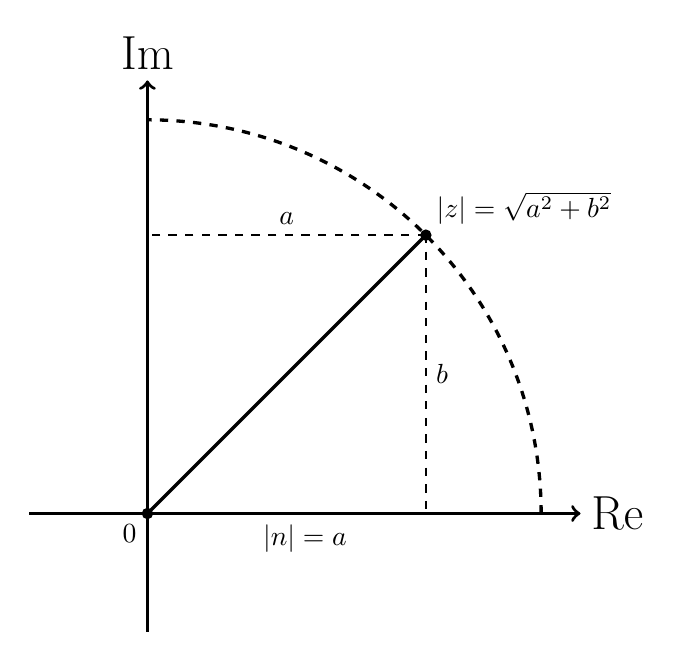
\begin{tikzpicture}

% Define the radius
\def\radius{5}
\def\angle{45} % Angle in degrees

% Convert angle to radians for cos and sin functions
\pgfmathsetmacro\x{\radius * cos(\angle)}
\pgfmathsetmacro\y{\radius * sin(\angle)}

% Draw axes
\draw[very thick, ->] (-1.5,0) -- (\radius+0.5,0) node[right] {\LARGE Re} node[midway, below] {$|n| = a$};
\draw[very thick, ->] (0,-1.5) -- (0,\radius+0.5) node[above] {\LARGE Im};

% Draw complex number
\coordinate (A) at (\x,\y);
\draw[very thick, fill] (A) circle [radius=0.05] node[above right] {$|z| = \sqrt{a^2 + b^2}$};

% Draw origin
\coordinate (O) at (0,0);
\draw[very thick, fill] (O) circle [radius=0.05] node[below left] {$0$};

% Draw line from origin to complex number
\draw[-, very thick] (O) -- (A) node[midway,above, sloped]{};

% Draw quarter circle arc
\draw[very thick, dashed] (\radius,0) arc[start angle=0, end angle=90, radius=\radius];

% Draw right-angle triangle
\draw[thick, dashed] (A) -- (\x,0) node[midway, right] {$b$};
\draw[thick, dashed] (A) -- (0,\y) node[midway, above] {$a$};

\end{tikzpicture}


\caption{Calculation of the magnitude of the complex coefficients as the euclidean distance from $0 + 0i$, as it relates to the implicit magnitude of real-valued data ($|n|=a$).}
\label{fig:imag}
\end{figure}

Significance testing follows as normally, and the complex characteristics of the data are preserved for the subsequent visualization step. The loadings of the reconstructed matrices for each experimental factor are projected using summed reconstruction and error terms to calculate the scores for the ASCA model according to an arbitrary factor $A$:
%
\begin{align}\label{eq:asca}
    \mathbf{T}_A\mathbf{P}_A^H = \mathbf{X}_A \\
    \mathbf{T}^*_A = (\mathbf{X}_A + \mathbf{E})\mathbf{P}_A
\end{align}
%
\noindent where the scores and loadings matrices $\mathbf{T}_A$ and $\mathbf{P}_A$ are respectively $N \times R$, and $M \times R$ complex matrices, with $\mathbf{P}_A^H$ representing the Hermitian of the loadings matrix $\mathbf{P}_A$. In the frequency domain, the loadings $\mathbf{P}_A$ may not be particularly easy to interpret as an abstraction of the original data in the time series. But the loadings can be transformed back into the time domain without sacrificing the least-squares solution to the GLM-like (General least squares, similar to ANOVA under certain conditions - see Section \ref{sec:glm}) problem as in Equation \ref{eq:least_squares}. Consider $\mathbf{X}_m$ as the time-domain representation of a designed experimental dataset with one significant factor, and $\mathbf{X}_k$ as the corresponding frequency domain representation. Equations \ref{eq:fft} and \ref{eq:ifft} can be represented by the $M\times M$ linear transformation $\mathbf{F}$ for the Discrete Fourier Transform (DFT), and $\frac{1}{M}\mathbf{F}^{-H} = \mathbf{F}^{-1}$ for the corresponding inverse scaled by the number of observations, $M$. It follows that:

\begin{align}\label{eq:least_squares}
    \mathbf{X}_k = \mathbf{X}_m\mathbf{F}\\
    \mathbf{X}_m = \mathbf{X}_k\mathbf{F}^{-1}\\
    \mathbf{X}_k = \mathbf{T}\mathbf{P}^H + \mathbf{E}\\
    \mathbf{X}_m = \left(\mathbf{T}\mathbf{P}^H + \mathbf{E}\right)\mathbf{F}^{-1}\\
    \mathbf{X}_m = \mathbf{T}\left(\mathbf{P}^H\mathbf{F}^{-1}\right) + \mathbf{E}\mathbf{F}^{-1}
\end{align}

And so the transform of the loadings from the frequency domain encompass similar variance as a function of the linear transformation $\mathbf{F}$, and can be interpreted following the inverse transform. Additionally, the reconstructions of $\mathbf{X}$ according to the different experimental factors may be transformed back to the time domain for an inspection of the different peaks responsible for affecting the level separations. Inspecting the equations shows that the relationship is \textit{least squares} in the frequency domain, which is not to say the same relationship holds in the time domain (in instances where there is significant peak drift). Following the reconstruction of the data according to the \textit{treatment} factor in Figure \ref{fig:freq_treat}, the varying width of the lines illustrate this in regards to peak drift in the time domain.

\subsection{Experimental Data and Methodology}

Data from a study measuring the changes in chemical profiles of the red flour beetle \textit{Tribolium castaneum}, as a function of immune stimulation. The motivation for the original study \cite{lo2023immune} (associated data was collected from the corresponding MetaboLights repository (\url{https://www.ebi.ac.uk/metabolights/editor/MTBLS2277}) was to investigate how the insects communicate via chemical signalling in response to environmental stressors. One of the two experimental datasets for this design was used in this example, which analysed stink glad secretions 24h and 72h following the absence of any exposure to environmental stressors, exposure to physical wounding via sterile PBS injection, and exposure to inactive \textit{Bacilius thuringiensis bv. tenebrionis}. Each sample represents the stink gland secretions of one individual, collected through chemical extraction and analysed using GC-FID. In addition to the sex of the individuals being a factor in the design, the order in which the samples were run were considered as an additional experimental variable which is presumed not to be significant. The contributions of each factor to the overall variance in the model is summarized as:

\begin{equation}\label{eq:GLM}
    \mathbf{X} = \mathbf{T} + \mathbf{R} + \mathbf{S} + \mathbf{O} + \mathbf{E}
\end{equation}

\noindent which encompasses $\mathbf{T}$, $\mathbf{R}$, $\mathbf{S}$, and $\mathbf{O}$ as the reconstructed matrices for ``Time'', ``Treatment'', ``Sex'', and ``Order'' respectively. 

All experimental data were analyzed using a modified variant of the MEDA Toolbox (to handle complex data) on MATLAB 2024a. The calculations were performed on system running Ubuntu 22.04.4 LTS with an Intel i9-1400K 32 core CPU, two parallel NVIDIA GeForce RTX 4070 GPUs and 128 GB of RAM. Experimental meta-data were converted to numerical format using Python. All code used in the analysis are available in the repository \url{https://github.com/CoDaSLab/fftasca_gcfid}.

\section{Results and Discussion}

\subsection{Analysis of a synthetic dataset}\label{sec:2.1}

Missing data presents a considerable challenge for comparison. In cases where there is a zero present, whether or not this zero represents a value of zero, or a peak that was improperly integrated is ultimately left to the discretion of the integration software, and the hard thresholds for peak detection included as part of the meta-parameters prior to analysis. It is therefore difficult to compare two ``known-unknowns" much less the features that are not apparent in the peak table at all: the ``unknown-unknowns" \cite{rumsfeld2002}, and a reference against a dataset whose characteristics are known \textit{a-priori} is therefore sought.

To test the accuracy of the ASCA model in the frequency domain, several synthetic datasets were prepared with varying levels of peak drift between samples to illustrate the relative robustness of acquisition level analyses versus the proposed frequency-domain analysis. A very simple multivariate experimental design was used to generate the amplitude of several different peaks, whose relative position was modified as per the ``jitter level''. The relative \textit{p}-values were transformed into their corresponding \textit{z}-values assuming an approximately normal distribution for generation of accurate confidence intervals per jitter level. The synthetic GC-FID dataset was made using an approach to simulate multivariate relationships \cite{Camacho2016} for one significant linear factor which is measured for consistency in Figure \ref{eq:sig_test}. The output of this routine was used to inform the amplitude of 5 Gaussian peaks, with an additional 5 whose amplitudes were randomly generated. Across each simulated samples' 5000 acquisitions, the Gaussian peak widths of $4\sigma$ were nominally sampled 20 times, which is typical for such data. Random peak drift, or ``jitter'' on the order of 0 to 50 acquisitions was generated while preserving the relative peak order, and at each instance an parallel GLM analysis was performed on the raw data (time), versus a similar analysis performed following an FFT transformation (frequency). At each level, a randomly generated synthetic dataset was created for $n=10$ replicates. The synthetic data can be seen in Appendix \ref{sec:vis}.

\begin{figure}[hbt!]
    \centering
    \includegraphics[width=0.9\linewidth]{comparison.pdf}
    \caption{As shown by the results of this analysis, as the jitter in the data increases, the hypothesis testing step in the parGLM (parallel GLM - for multivariate analysis) step using the time-domain data becomes much less sensitive. However, following pre-processing using an FFT analysis the results are much more consistent.}
    \label{fig:compare}
\end{figure}

The results in Figure \ref{fig:compare} suggest that the evidence for significance of the one linear factor is better preserved as a function of increasing jitter, versus the time-series analysis. It was observed that when the order of the peaks changed, this relationship was no longer valid, which indicates that this method is still not appropriate for truly heterogeneous data for GC-FID instrumentation. This is because there is no distinguishing characteristics for each peak beyond its position in chromatogram, and this information is lost when it may be indicated as another chemical factor entirely. Nonetheless, the results suggest its applicability to well-controlled experimental data with relatively minor drift in retention times that do not affect the overall topology of the data.

\subsection{Analysis of real data}

Since it has already been proven that the analysis in the frequency domain is equivalent in its findings to the analysis in the time domain under ideal conditions, FFT-ASCA is next applied to a real dataset whose characteristics are not known ahead of time. As mentioned in Section \ref{sec:2.1}, the peak table contains missing values that could be either \textit{unknown} (i.e. not properly integrated), or truly absent. This may be the case when the peak is found in some samples, but not others. Additionally, for extremely scarce components that are not included in the peak table at all, these components may have an effect on the model that is entirely absent in the peak table comparison.  

The results of several ASCA models are shown below in Table \ref{tb:results}, using the raw chromatographic signals from \cite{lo2023immune}.  The peak tables provided as part of the original study were mean-centred. The effect of missing values in the peak table data were examined by performing the ASCA analysis on the data with and without a permutational conditional mean replacement strategy for minimizing the effect of missing data on measuring the effect of different experimental factors. In short, for each permutation, the missing values are replaced with the apparent \textit{cell mean} as the shifted data presents relative to the experimental design matrix which is kept constant. All zeros were presumed to be missing values.

For each GLM analysis, all binary interacting terms were examined before being ``trimmed'' in a subsequent analysis where only the previously indicated terms were included in the model. Interacting terms whose linear factors were not indicated as significant were not considered, except for interaction between Time and Treatment which is close to the cutoff for $\alpha = 0.05$ and further demonstrates consistency between the peak table analysis accounting for missing data, and the FFT-ASCA results - listed as \textbf{FFT, mean-centred} in Table \ref{tb:results}, where the similar evidence of significance for each of the experimental factors is highlighted in blue. 

\begin{table} % It is hard to append tables - if the results are refreshed make sure that the \begin and \end terms are removed. You may have to re-label some things.
\begin{tabular}{llllllll}
\textbf{Peak Table w/ zeros} & SumSq & PercSumSq & df & MeanSq & F & Pvalue \\ 
 \hline 
Mean & 2.2e+08 & 67.1 & 1 & 2.2e+08 & -- & -- \\ 
Time-1 & 7.53e+05 & 0.229 & 1 & 7.53e+05 & 0.747 & 0.412 \\ 
Treatment-2 & 9.45e+06 & 2.88 & 2 & 4.73e+06 & 4.69 & \textbf{0.00999} \\ 
Sex-3 & 1e+07 & 3.06 & 1 & 1e+07 & 9.96 & \textbf{0.002} \\ 
Order-4 & 5.26e+06 & 1.6 & 7 & 7.51e+05 & 0.745 & 0.675 \\ 
Interaction 1-2 & 4.19e+06 & 1.27 & 2 & 2.09e+06 & 2.08 & 0.113 \\ 
Residuals & 7.86e+07 & 23.9 & 78 & 1.01e+06 & -- & -- \\ 
Total & 3.29e+08 & 100 & 92 & 3.57e+06 & -- & -- \\ 

 \\
 \textbf{Peak Table pCMR}& SumSq & PercSumSq & df & MeanSq & F & Pvalue \\ 
 \hline 
Mean & 5.2e+03 & 68.6 & 1 & 5.2e+03 & -- & -- \\ 
Time-1 & 80.9 & 1.07 & 1 & 80.9 & 3.67 & \textbf{0.022} \\ 
Treatment-2 & 115 & 1.52 & 2 & 57.5 & 2.6 & \textbf{0.018} \\ 
Sex-3 & 180 & 2.38 & 1 & 180 & 8.17 & \textbf{0.000999} \\ 
Order-4 & 161 & 2.13 & 7 & 23 & 1.04 & 0.381 \\ 
Interaction 1 & 92.1 & 1.22 & 2 & 46.1 & 2.09 & 0.0569 \\ 
Residuals & 1.72e+03 & 22.7 & 78 & 22.1 & -- & -- \\ 
Total & 7.58e+03 & 100 & 92 & 82.4 & -- & -- \\ 

 \\ 
 \textbf{FFT, mean-centred}& SumSq & PercSumSq & df & MeanSq & F & Pvalue \\ 
 \hline 
Mean & 5.84e+14 & 5.09 & 1 & 5.84e+14 & -- & -- \\ 
Time-1 & 1.54e+15 & 13.4 & 1 & 1.54e+15 & 19.5 & \textbf{0.000999} \\ 
Treatment-2 & 7.79e+14 & 6.78 & 2 & 3.89e+14 & 4.92 & \textbf{0.00599} \\ 
Sex-3 & 8.7e+14 & 7.57 & 1 & 8.7e+14 & 11 & \textbf{0.00599} \\ 
Order-4 & 7.13e+14 & 6.2 & 7 & 1.02e+14 & 1.29 & 0.25 \\ 
Interaction 1-2 & 4.51e+14 & 3.93 & 2 & 2.26e+14 & 2.85 & 0.0569 \\ 
Residuals & 6.49e+15 & 56.5 & 82 & 7.92e+13 & -- & -- \\ 
Total & 1.15e+16 & 100 & 96 & 1.2e+14 & -- & -- \\ 
\end{tabular} 
 \\

\caption{Results of GLM analyses of the experimental factors versus the different representations of the multivariate data. Beginning with the un-altered peak table, followed by the zero-handling GLM with permutational conditional mean replacement (pCMR) \cite{pCMR}, and then the mean-centred frequency domain GLM analysis which contains no missing information. P-values below 0.05 are shown in bold.}
\label{tb:results}

\end{table}

From the results of Table \ref{tb:results} it is clear from the apparent significance of the experimental factors, that the presence of zeros and/or missing data has a profound effect on the resulting interpretation of the data. In the peak table representation, failure to account for zeros neglects to demonstrate the significance of the time factor, and suppresses the relative weight of the interacting term. Because the peak table representation relies on an intermediate step to integrate the peaks, it is impossible to know which zeros are truly absent from the data, and which zeros have failed to be integrated by the software. However it is worth noting that a similar treatment in the time and frequency domains yields similar results when the zeros are accounted for by the permutational cell mean replacement routine. In cases where the chemical factors are truly absent from one class, they are nonetheless replaced with the average, or expected value according to samples with similar experimental characteristics. The \textit{p}-values are driven by the frequency with which the simulated \textit{null} hypothesis exceeds the apparent test statistic, which is in turn driven by the difference between experimental levels over variation within samples with similar characteristics. And so for instances where a chemical component is truly absent from one set of samples, whether or not the value is represented by zero, or the imputed value per \textit{pCMR} (permutational cell mean replacement) is not expected to be particularly consequential if the difference is continually observed over several permutations of the original data.

Figures \ref{fig:figure1} and \ref{fig:figure2} demonstrate that the scores from the analysis appear to be more consistent using FFT-ASCA than by using ASCA on the peak table information alone, and the discrete peak loadings in Figure \ref{fig:figure5} show some similarity to the continuous, inverse transformed loadings in Figure \ref{fig:figure6}. This further highlights that pCMR is currently only capable of handling issues with significance testing, and that visualization is still strongly influenced by the presence of missing data.  Figures \ref{fig:figure3} and \ref{fig:figure4} represent the complex loadings of the data that are impossible to interpret, but whose inverse transformation corresponds to meaningful chemical variability in Figure \ref{fig:figure6}.

\subsection{ASCA}

From Equation \ref{eq:asca} the following \textit{post-hoc} visualizations of the data were performed in agreement with significance testing results. The factor ``Time'' was indicated as significant only after correcting for missing values in the peak table data, but this routine does not affect the factorization and visualization by ASCA (only the inference), which does not yield especially interpretable results (see Figure \ref{fig:figure1}). 

\begin{figure}[hbtp!]
    \centering
    \begin{subfigure}[b]{0.45\textwidth}
        \centering
        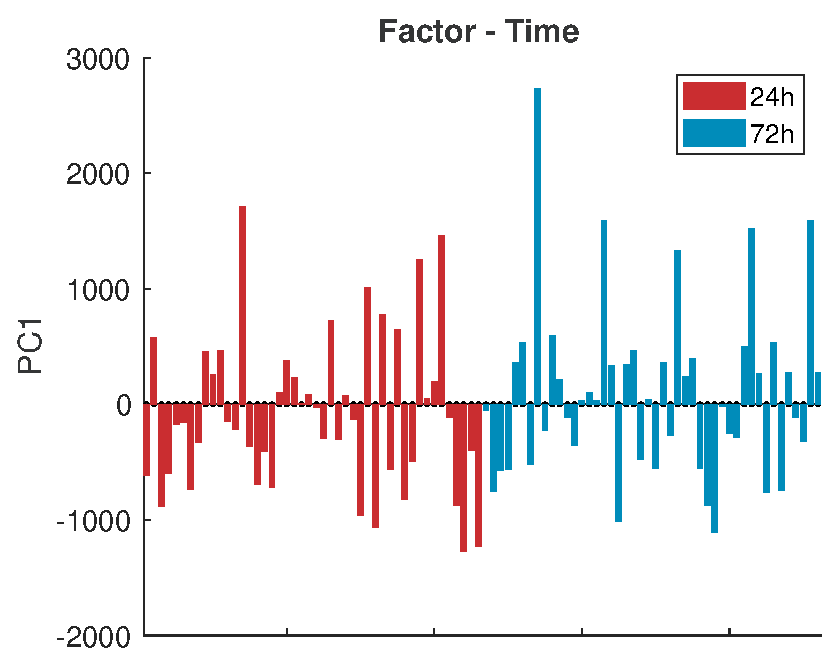
\includegraphics[width=\textwidth]{peak_time.eps}
        \caption{Peak table PCA scores of factor ``Time''.}
        \label{fig:figure1}
    \end{subfigure}
    \hfill
    \begin{subfigure}[b]{0.45\textwidth}
        \centering
        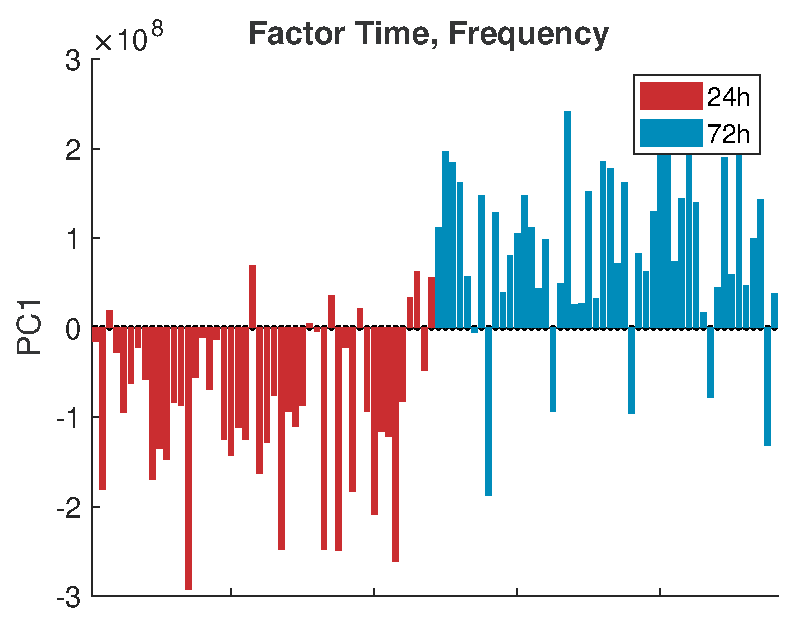
\includegraphics[width=\textwidth]{freq_time_mn.eps}
        \caption{Real-valued PCA scores for factor ``Time'' from FFT transformed data. Mean-centred.}
        \label{fig:figure2}
    \end{subfigure}
    
    \vfill
    
    \begin{subfigure}[b]{0.45\textwidth}
        \centering
        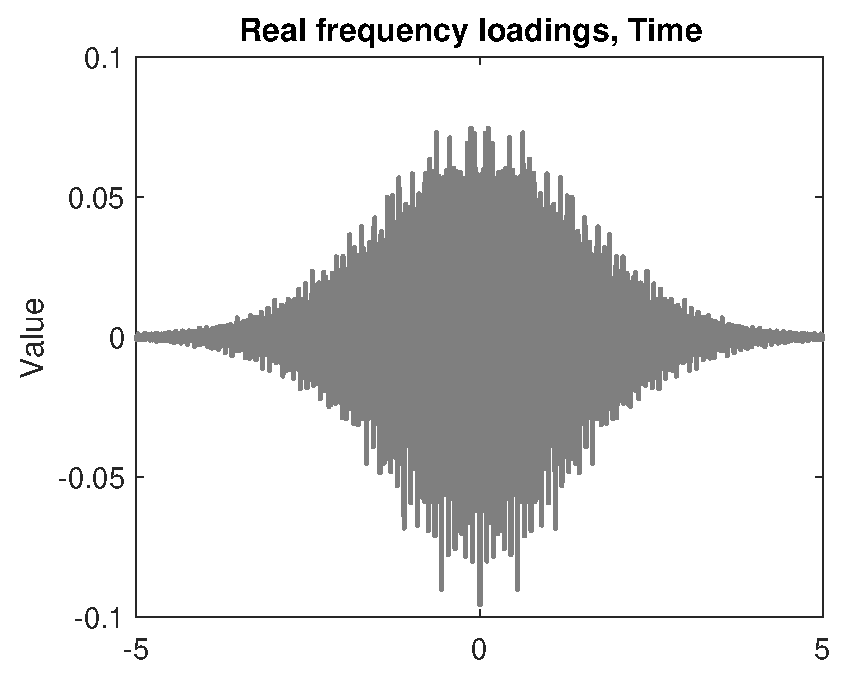
\includegraphics[width=\textwidth]{freq_loads_time_real.eps}
        \caption{Loadings for factor "Time" from the peak table representation of the data. 26 targeted metabolites were included in the analysis.}
        \label{fig:figure3}
    \end{subfigure}
    \hfill
    \begin{subfigure}[b]{0.45\textwidth}
        \centering
        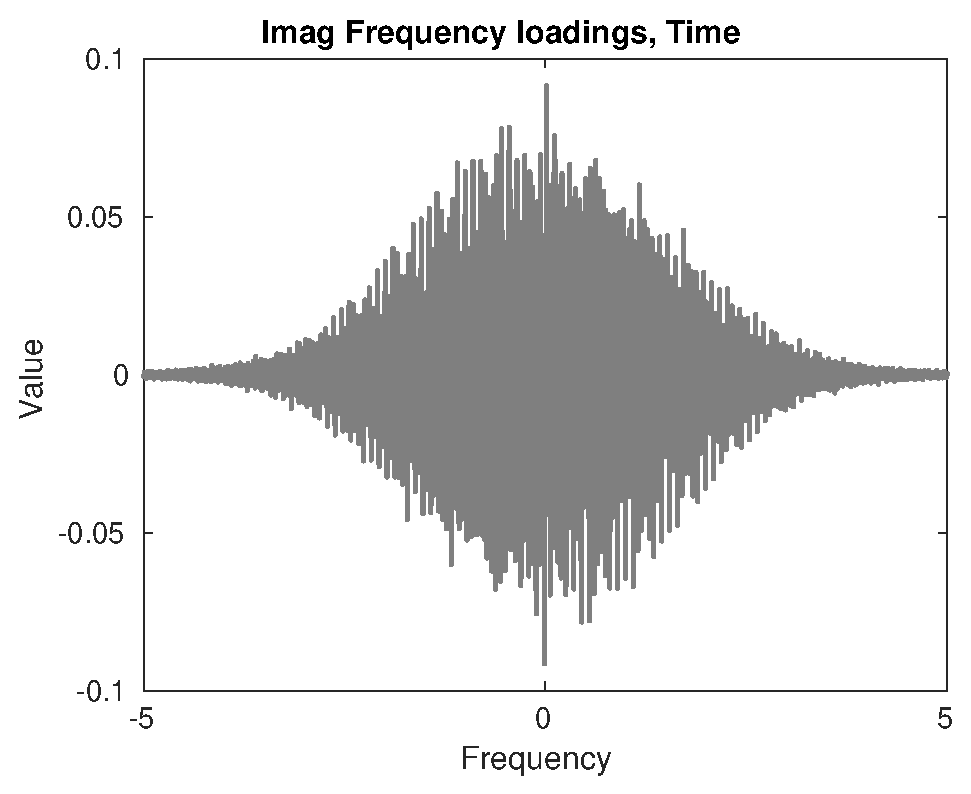
\includegraphics[width=\textwidth]{freq_loads_time_imag.eps}
        \caption{Complex-valued loadings in the frequency domain for factor ``Time''.}
        \label{fig:figure4}
    \end{subfigure}
    \vfill

\begin{subfigure}[b]{0.45\textwidth}
        \centering
        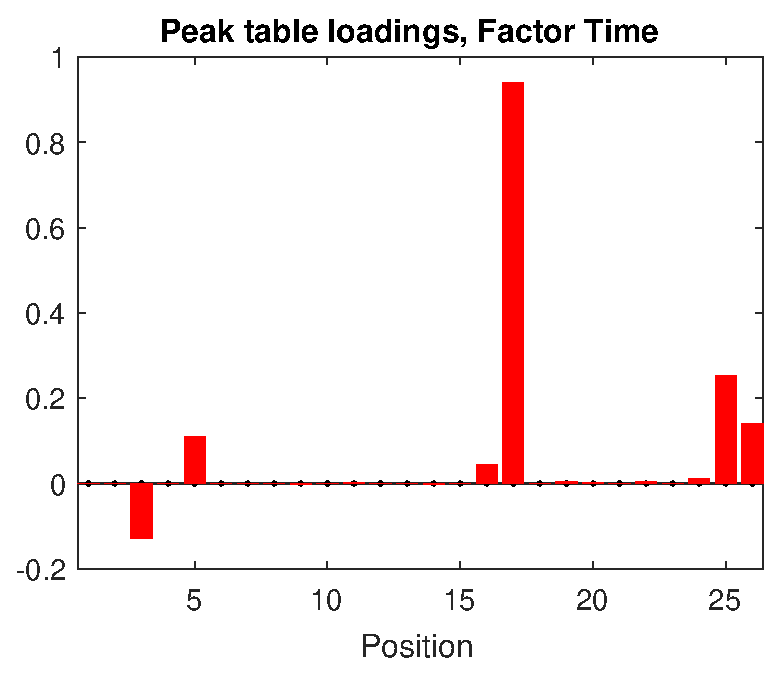
\includegraphics[width=\textwidth]{peak_loads_time.eps}
        \caption{Real-valued loadings in the time domain for factor ``Time''.}
        \label{fig:figure5}
    \end{subfigure}
    \hfill
    \begin{subfigure}[b]{0.45\textwidth}
        \centering
        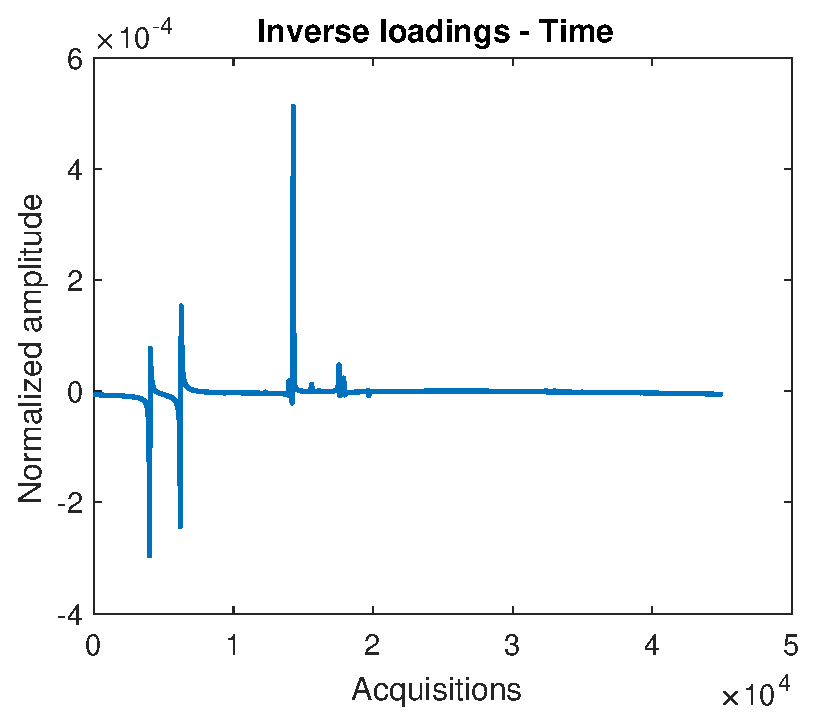
\includegraphics[width=\textwidth]{time_peaks.eps}
        \caption{Real-valued loadings in the time domain for factor ``Time''.}
        \label{fig:figure6}
    \end{subfigure}
    \caption{ASCA results for the peak table analysis, as well as the frequency-domain analysis. The real-valued scores in the frequency domain are more consistent (Figure \ref{fig:figure2}, versus Figure \ref{fig:figure1}), but the loadings themselves are less interpretable (Figures \ref{fig:figure3} and \ref{fig:figure4}). They can however be transformed back into the time domain, as shown in Figure \ref{fig:figure6}.}
    \label{fig:subfigures}
\end{figure}

In addition to analyzing the loadings, the individual factor matrices themselves can be transformed back into the time domain for  inspection via Equation \ref{eq:ifft}. This type of analysis shows that the GLM performed on the frequency domain, as an abstraction of the original, raw data still corresponds to real-valued chemical components. An example is shown in Figure \ref{fig:freq_treat}, where a single chemical factor with evidence of statistical significance in the frequency domain, is clearly differentiated according to its levels in the time domain.

\begin{figure}[hbt!]
    \centering
    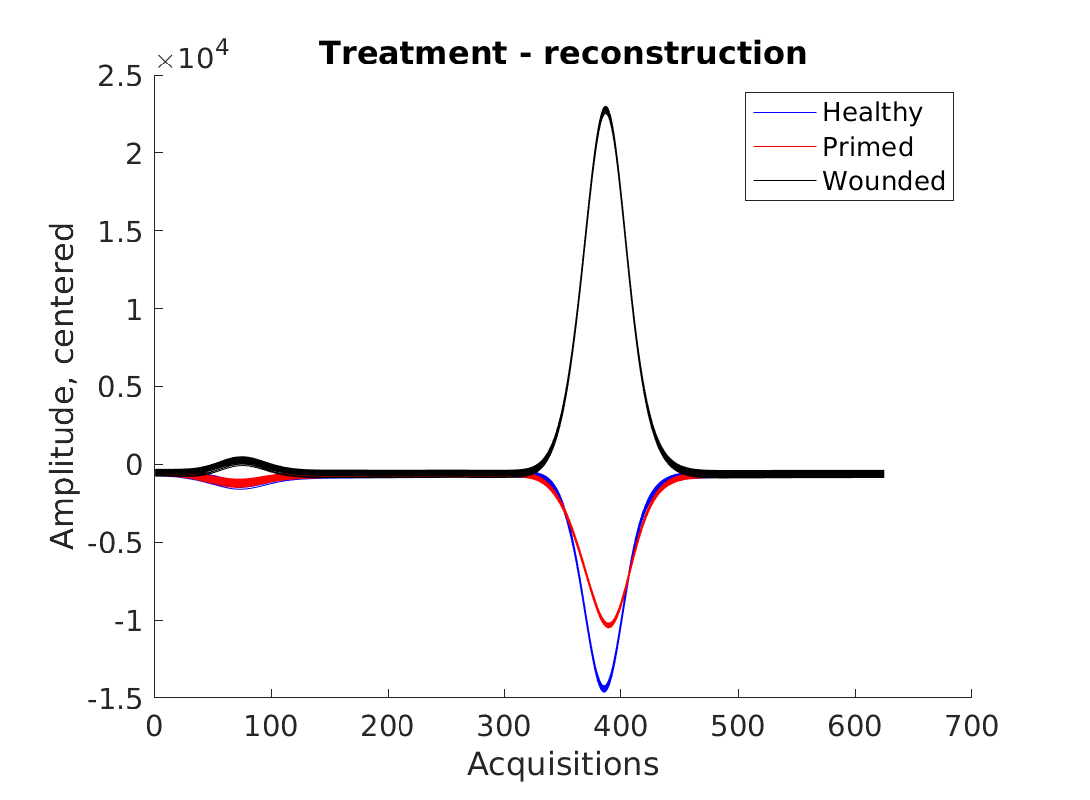
\includegraphics[width=0.9\linewidth]{time_treat.eps}
    \caption{Time-domain reconstruction of factor ``Treatment'' where the levels are clearly differentiated. This is a reconstruction of $\mathbf{X}_{treatment}$ using the inverse transform in Equation \ref{eq:least_squares}.}
    \label{fig:freq_treat}
\end{figure}


\section{Conclusions}

FFT-ASCA analyses appear to subvert some common problems with pre-processing of chromatographic data. In the experimental dataset, the presence of missing values in the peak table was shown to have a strong effect on the resulting interpretation. A transformation of the raw data itself however to a series of fully-populated Fourier coefficients offers similar insight into the analysis following missing value correction, and for a similar level of interpretability. While simple, this method offers new ways of analyzing chromatographic data, in a manner that relies on fewer meta-parameters for feature engineering and extraction prior to the analysis step. Although this technique has not been definitely proven to out-perform traditional methods for analyzing chromatographic data in all cases, this demonstration is representative of a number of issues faced by laboratory scientists handling and interpreting chromatographic data. GC-FID is not commonly used for metabolomics-type work, but this type of methodology is easily generalized to hyphenated and/or multi-modal separations using similar extensions of multivariate statistics to tensor analysis that have already been widely discussed in literature \cite{koleini2023complementary}. 

\section{Acknowledgements}

This work was supported by the Agencia Estatal de Investigación in Spain for call no. MCIN/AEI/10.13039/501100011033 and grant no. PID2023-1523010B-IOO (MuSTARD). Michael Sorochan Armstrong has received funding from the European Union's Horizon Europe research and innovation programme under the Marie Skłodowska-Curie grant agreement Meta Analyses of Heterogeneous Omics Data (MAHOD) no. 101106986 .

%% If you have bibdatabase file and want bibtex to generate the
%% bibitems, please use
%%
\bibliographystyle{ieeetr}
\bibliography{cas-refs}

\appendix

\section{Visualizations of Synthetic Data}\label{sec:vis}

The following visualizations are used to demonstrate the extent of peak drift using 3 samples for the first 2000 acquisitions.

\begin{figure}[h]
    \centering
    \includegraphics[width=0.75\textwidth]{figures/jitter_illustration1.pdf}
    \caption{Three samples with no jitter}
    \label{fig:figure1}
\end{figure}

% Figure 2
\begin{figure}[h]
    \centering
    \includegraphics[width=0.75\textwidth]{figures/jitter_illustration2.pdf}
    \caption{3 samples with jitter level 2}
    \label{fig:figure2}
\end{figure}

% Figure 3
\begin{figure}[h]
    \centering
    \includegraphics[width=0.75\textwidth]{figures/jitter_illustration3.pdf}
    \caption{3 samples for jitter level 3}
    \label{fig:figure3}
\end{figure}

% Figure 4
\begin{figure}[h]
    \centering
    \includegraphics[width=0.75\textwidth]{figures/jitter_illustration4.pdf}
    \caption{3 samples for jitter level 4}
    \label{fig:figure4}
\end{figure}

% Figure 5
\begin{figure}[h]
    \centering
    \includegraphics[width=0.75\textwidth]{figures/jitter_illustration5.pdf}
    \caption{3 samples for jitter level 5}
    \label{fig:figure5}
\end{figure}

% Figure 6
\begin{figure}[h]
    \centering
    \includegraphics[width=0.75\textwidth]{figures/jitter_illustration6.pdf}
    \caption{3 samples for jitter level 6}
    \label{fig:figure6}
\end{figure}

% Figure 7
\begin{figure}[h]
    \centering
    \includegraphics[width=0.75\textwidth]{figures/jitter_illustration7.pdf}
    \caption{3 samples for jitter level 7}
    \label{fig:figure7}
\end{figure}

% Figure 8
\begin{figure}[h]
    \centering
    \includegraphics[width=0.75\textwidth]{figures/jitter_illustration8.pdf}
    \caption{3 samples for jitter level 8}
    \label{fig:figure8}
\end{figure}

% Figure 9
\begin{figure}[h]
    \centering
    \includegraphics[width=0.75\textwidth]{figures/jitter_illustration9.pdf}
    \caption{3 samples for jitter level 9}
    \label{fig:figure9}
\end{figure}

% Figure 10
\begin{figure}[h]
    \centering
    \includegraphics[width=0.75\textwidth]{figures/jitter_illustration10.pdf}
    \caption{3 samples for jitter level 10}
    \label{fig:figure10}
\end{figure}

% Figure 11
\begin{figure}[h]
    \centering
    \includegraphics[width=0.75\textwidth]{figures/jitter_illustration11.pdf}
    \caption{3 samples for jitter level 11}
    \label{fig:figure11}
\end{figure}


%% else use the following coding to input the bibitems directly in the
%% TeX file.

% \begin{thebibliography}{00}

% %% \bibitem{label}
% %% Text of bibliographic item

% \bibitem{}

% \end{thebibliography}
\end{document}
\endinput
%%
%% End of file `elsarticle-template-num.tex'.
